% Template last modified by Jake Hart; please contact course staff if you have any questions regarding using this template

\documentclass{cisXXX} % You must have the cisXXX .cls file in your project or working directory (i.e. the same directory as this document) 

\HWauthor{Zeyu Zhao}{zhaozeyu@seas.upenn.edu} % Put your name and Penn email on this line
\HWno{12} % Enter the number of the homework you are working on
\HWcourse{ESE 303} % Enter the course department and number here
%\HWpartner{Paul Brown} % If your class allows group work, put your partners here
%\HWpartner{Amelia Earhart} % Otherwise, delete or comment these lines 
\usepackage{amsmath}
\usepackage{amsfonts}
% code
\usepackage{color}
\usepackage[framed,numbered,autolinebreaks,useliterate]{mcode}
\usepackage{graphicx}
\definecolor{dkgreen}{rgb}{0,0.6,0}
\definecolor{gray}{rgb}{0.5,0.5,0.5}
\definecolor{mauve}{rgb}{0.58,0,0.82}
\begin{document}
\maketitle
\HWproblem
Assume otherwise, if an arbitrage opportunity exists, it means that no matter the outcome of the game, the bidder always walks home with positive amounts of money. 

We employ the famously announced equation by Prof. Ribeiro in class, that if there exists an arbitrage, then the odds of all possible outcomes (in this example say $\{a, b, c\}$) must satisfies:
$$
1/a + 1/b + 1/c < 1
$$
We verify that the arbitrage doesn't exist:
$$
1/6.6 + 1/8.1 + 1/1.2 = 1.10830527497 > 1
$$
Therefore the arbitrage opportunity does not exist.
\HWproblem
There just cannot be an arbitrage when the return of one of the outcomes is less than 1. Specifically, if \textbf{Other} happens, then we get back at most 0.3 of what we bid. Therefore no arbitrage is possible. However, we can sort of do the best we can by playing the best odds from each booker: 

Specifically, bidding on Brazil with booker 1, on Spain with booker 3 and on Other with booker 2 yields the best return rate. Suppose we know the true probability of which team winning, which is $p$ of Brazil, $q$ of Spain, and $1-p-q$ of Other. Then we invest $x$ on Brazil, $y$ on Spain, and $1 - x -y$ on Other.

Then the expected payoff is $P = p * (5.6x - 1) + q*(7.4y - 1) + (1-p-q) * (0.3 * (1 - x - y) - 1)$ 
Then we maximize with respect to $x, y$. The $x$ derivative is $5.9p + 0.3q -0.3$; the $y$ derivative is $0.3p + 7.7q -0.3$. Suppose $p = 0.2, q = 0.3$. Then the max is $(x, y) = (0, 1)$.
A result of this optimization is shown in Figure \ref{fig:Maximize}.
\begin{figure}
  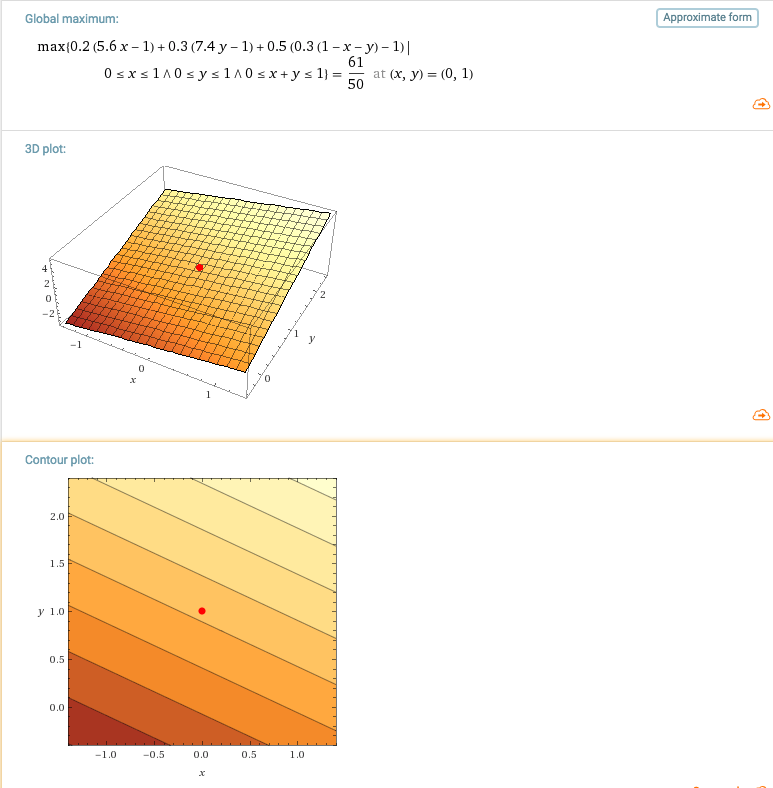
\includegraphics[width=\linewidth]{maximize.png}
  \caption{Wolfram Alpha Maximizer when $p = 0.2, q = 0.3$.}
  \label{fig:Maximize}
\end{figure}

\end{document}